\documentclass[review]{elsarticle}

\makeatletter
\def\@author#1{\g@addto@macro\elsauthors{\normalsize%
    \def\baselinestretch{1}%
    \upshape\authorsep#1\unskip\textsuperscript{%
      \ifx\@fnmark\@empty\else\unskip\sep\@fnmark\let\sep=,\fi
      \ifx\@corref\@empty\else\unskip\sep\@corref\let\sep=,\fi
      }%
    \def\authorsep{\unskip,\space}%
    \global\let\@fnmark\@empty
    \global\let\@corref\@empty  %% Added
    \global\let\sep\@empty}%
    \@eadauthor={#1}
}
\makeatother

\usepackage{lineno}
\usepackage{color}
\usepackage[hidelinks]{hyperref}
\usepackage{graphicx}
\usepackage{caption}
\usepackage{epstopdf}
\usepackage{multirow}
\usepackage{lineno}
\usepackage{amssymb}
\usepackage{pgfplots}
\usepackage{tikz}
\usepackage{subcaption}
\usepackage{rotating}
\usepackage{threeparttable}
\usetikzlibrary{matrix}
\usetikzlibrary{spy}
\usepgfplotslibrary{groupplots}
\pgfplotsset{compat=newest}
\graphicspath{ {./figures/} }



\modulolinenumbers[5]
\journal{Journal of \LaTeX\ Templates}

%%%%%%%%%%%%%%%%%%%%%%%
%% Elsevier bibliography styles
%%%%%%%%%%%%%%%%%%%%%%%
%% To change the style, put a % in front of the second line of the current style and
%% remove the % from the second line of the style you would like to use.
%%%%%%%%%%%%%%%%%%%%%%%

%% Numbered
%\bibliographystyle{model1-num-names}

%% Numbered without titles
%\bibliographystyle{model1a-num-names}

%% Harvard
%\bibliographystyle{model2-names.bst}\biboptions{authoryear}

%% Vancouver numbered
%\usepackage{numcompress}\bibliographystyle{model3-num-names}

%% Vancouver name/year
%\usepackage{numcompress}\bibliographystyle{model4-names}\biboptions{authoryear}

%% APA style
%\bibliographystyle{model5-names}\biboptions{authoryear}

%% AMA style
%\usepackage{numcompress}\bibliographystyle{model6-num-names}

%% `Elsevier LaTeX' style
\bibliographystyle{elsarticle-num}
%%%%%%%%%%%%%%%%%%%%%%%

\begin{document}

\begin{frontmatter}

\title{Barreling formation during the axial compressive experiments on cubic
samples with orthotropic properties {\color{red} Preliminary title}}
%%\tnotetext[mytitlenote]{Fully documented templates are available in the
% elsarticle package on \href{http://www.ctan.org/tex-archive/macros/latex/contrib/elsarticle}{CTAN}.}

%% Group authors per affiliation:






%%\fntext[fn1]{This is the specimen author footnote.}
%%\fntext[fn2]{Another author footnote, but a little more longer.}
%%\fntext[fn3]{Yet another author footnote. Indeed, you can have any number of
% author footnotes.}

\author{Alexey Vorobyev\corref{cor1}}
\ead{alexey.vorobyev@angstrom.uu.se}

\cortext[cor1]{Corresponding author}

\author{Ingela Bjurhager}
\author{Nico P. van Dijk}
\author{Kristofer Gamstedt}

\address{Uppsala University, Division of Appplied Mechanics,
Uppsala, Sweden }



\begin{abstract}
This template helps you to create a properly formatted \LaTeX\ manuscript.
\end{abstract}

\begin{keyword}
Cubic samples\sep Compressive testing\sep Barrelling formation \sep
Wood
\end{keyword}

\end{frontmatter}

\linenumbers

\section{Introduction}

Characterisation of material stiffness parameters of orthotropic materials can
be challenging. In  careful design of wood structures, not only one parameter, but the full
orthotropic set of elastic parameters could be needed \cite{tsoumis1991science},
e.g. for finite-element modelling of wood joints that are locally subjected to a triaxial stress state.
Compressive experiments are considered to be one of the most common method for identifying engineering constants such as Young's
modulus, Poisson's ratio.The general approach is to measure material response
due to applied forces. The procedure is straitforward and easy to perform due to
simplicity of experimental installation and low requrements to speciemen
geometry. Standards such as ASTM \cite{standard1997d143},
\cite{johnson1983compression} are requiring the usage of rectangular prisms for
the compressive testing.
For rare wood material, e.g. archaeological wood, it is better to use cubic
samples \cite{ljungdahl2007transverse}.
This enables testing of the same sample several times and in different directions (radial, tangential, longitudinal) if the load is applied within the elastic range .
Disadvantages with compressive testing of cubes compared to tensile testing of dog-bone specimens, 
is that obtaining a pure compressive stress state is more complicated due to
inhomogeneous distribution of applied compression force due to geometrical
imperfections of test specimen \cite{Toftegaard1999849}.
Moreover, barrelling formation (Fig \ref{fig:barrelling}) in compressive
loading \cite{oldroyd1966stress}, due to the more or less restrained contact slip on the platens area, makes it difficult to assess the 
transverse deformations without having to resort to finite element modelling.
The Poisson�s ratios are thus more difficult to obtain directly from this kind
of loading.
Strain field measurements using digital image correlation are often required to
estimate the stiffness parameters accurately \cite{dahl2009planar,
majano2012test, ozyhar2013moisture}.
Additionally, the cylindrical orthotropy and curvature of the annual rings make the stress field even more non-uniform for large specimens. 
For too small specimens, the tested volume might not be representative, leading to a large scatter in measured stiffness. 
Nevertheless, compressive testing of wooden cubes is the reasonable choice of test method if the amount of available material is limited. 
Such problem arises when archaeological material is tetsted.

In 2012, a project with the aim of designing a new support structure for the
archaeological Vasa ship was initiated. The ship was capsized in 1628, and was salvaged in 1961. 
The waterlogged ship was impregnated with polyethylene glycol (PEG) in an extensive conservation process aiming to prevent deformation during drying. 
Extensive research during the last decades have found that the ship suffers from
agressive chemical degradation. Both the degradation \cite{bjurhager2012state} and the PEG impregnation \cite{ljungdahl2007transverse}
 have had a negative effect on the mechanical properties of the ship, which is in need of a better support. In 2012 a project with the aim of 
designing a new support structure for the fragile and soft ship was also initiated. For this task, the elastic, ultimate and creep properties of the 
Vasa oak need to be determined. Due to the limited access to material, cubic samples which can be tested several times is preferred.
In order to verify the results from the compressive experiments the effect of
barrelling was investifgated by the simulation using the Finate Element
Modelling (FEM).

Simulations of experiments in compression are not new. Previously compressive
experiments on prism samples with orthotropic material behavior were simulated
by \cite{Toftegaard1999849} in order to investigate the effect of geometrical imperfections on identification of engineering constants. 
He compared the simulated strain field to the measurements of strain gauges. 
Present work uses DSP in order to obtain the experimental strain field, which
contains strain data of observed area and not between two points as it is for the strain gauge. 
Chen \cite{Chen001} has simulated the behaviour of the specimen with geometrical
imperfections on a locked  seat during the compressive experiments
of composite materials. This is happening when platens of universal testing
machine (UTM) are locked and not automatically adjusted to sample geometry.
When a prism specimen is compressed between platens it contracts transversely.
Its surfaces bear heterogenious deformation that are resulting in barrelling
formation of the prism. 

%The purpose of experiment



Present work focuses on an investigation of
barrelling formation on two different mechanical types of materials. Additionally a comparison of three measuring techniques was made in order to identify the magnitude of error.
The results of presented investigaten can help to identify the ``true'' values
of material elastic parameters that can be obtainerd during compresive
experiments on the cubic samples. 

\begin{itemize}
\color{red}  



\item what problem was studied?
\item Introduction of the problem
\item Give the context of the problem
\item Reviews of previous works
\item Justification of work
\item Scopes and objectives
\item Interest the reader
\item Provide the transition to the rest
\end{itemize}

\section{Materials and Methods}

\begin{description}
\item{\textit{Experiment}}
\end{description}

A special care was taken in order to manufacture the specimens. Original sizes
of the sample was $25\times25\times25$ $mm$  The accuracy for parallelity
between the opposite edges of the cube was 0.01 $mm$. 

An Instron universal testing machine with 100 kN load cell was used to carry out static tests. 
Initial tests were conducted on dummy wood specimens in order to find the approximate elastic loading range for all specimen orientations.
The conventional way to measure strains is by using the built in measurement
system or strain gages. Nowadays, full field strain measurement techniques such
as digital speckle photography (DSP) \cite{synnergren1999stereoscopic} or
3D/stereo-digital image correlation (DIC) \cite{majano2012test} are used more
and more. The strain measurement using DIC has shown a good performance in
comparison to the traditional strain gauges \cite{huang2010optical},
\cite{xavier2012stereovision}. In our case, full-field displacements were observed with a digital-image correlation (DIC) equipment GOM Aramis stereo system 5M.
The distance to the measured object was 300 mm. Surface of specimen was spray
painted with speckles for better contrast. The applied force values were continuously recorded by the DIC system during testing, and stored together with the sampled images. The displacement rate was 0.5 mm per minute. 
The ambient conditions were $23\,^{\circ}{\rm C}$ and 51\% relative humidity.
All tests were performed without delay after the samples were removed from the conditioning storage container, so that the moisture content would essentially be the same as after conditioning. The measurement sampling frequency was 1 Hz. 
Every frame that was recorded by the DIC system was compared with the undeformed state in order to calculate the displacement and strain fields. 
The total surface area of interest used in image analysis was a centred square
of 625 $mm^\textsuperscript{2}$, where a uniform deformation field was found.
The chosen surface area of interest is marked by the dashed lin in Figure
\ref{fig:experiment}. The acquired strain fields were smoothed by averaging of
each data pixel with $3\times3$ surrounding pixels. The strains determined by
DIC in the loading direction was plotted against the applied stress, see Figure
\ref{fig:explot}.
Poisson's ratios $\nu_{ij}$ for all corresponding orthotropic planes were
calculated as a negative ratio between the average transverse $\varepsilon_{jj}$
(passive) and normal $\varepsilon_{ii}$ (compressive and active) strains.
The average transverse and normal strains measured along with normal ones were acquired with DIC technique.



\begin{figure}
    \centering
    \begin{subfigure}[b]{0.4\textwidth}
        \centering
        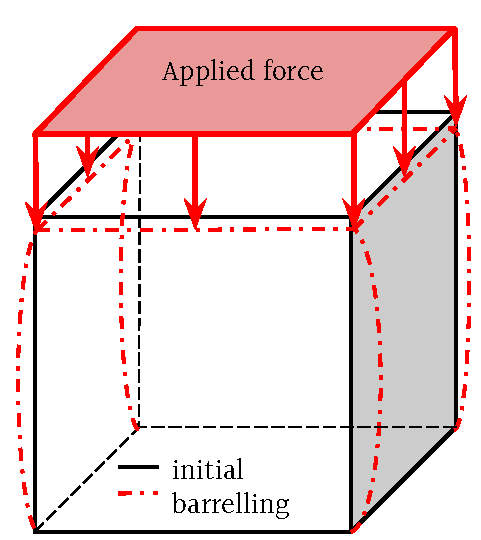
\includegraphics[width=\textwidth]{BarellingEffectZoomed.pdf}
        \caption{}
        \label{fig:barrelling}
    \end{subfigure}
    \hfill
    \begin{subfigure}[b]{0.4\textwidth}
        \centering
        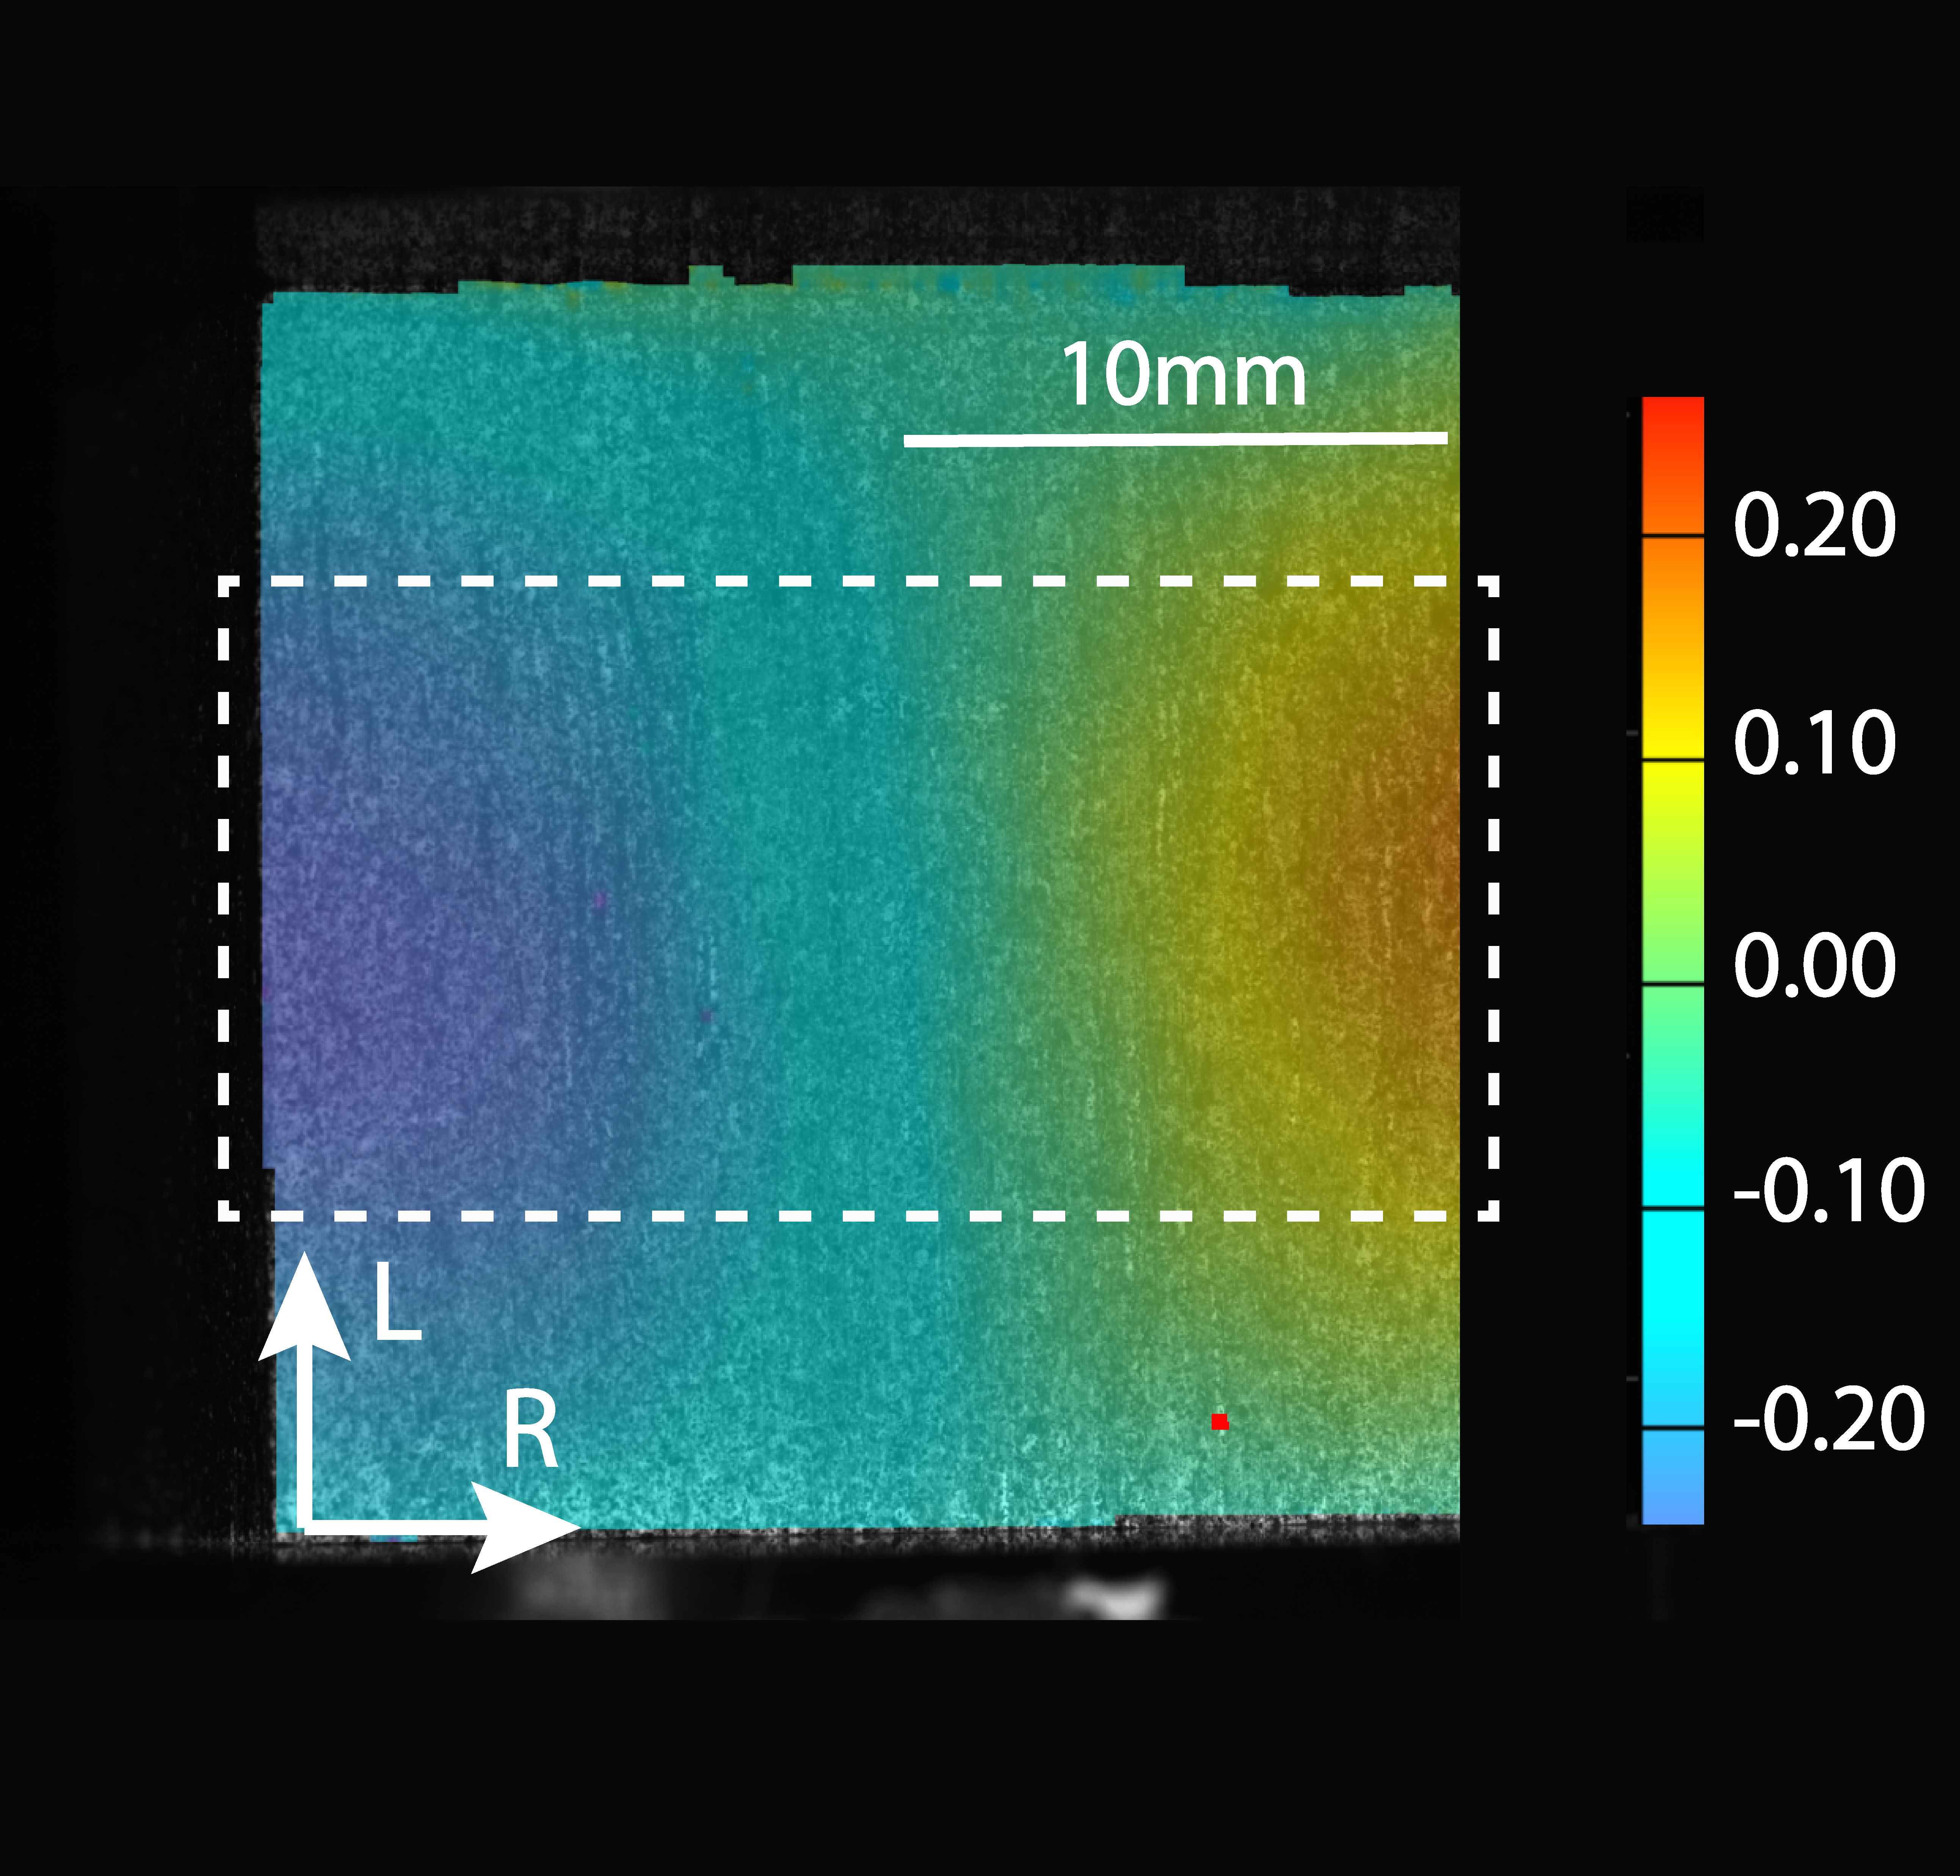
\includegraphics[width=\textwidth]{experiment.png}
        \caption{}
        \label{fig:experiment}
    \end{subfigure}
    \hfill
    \hspace*{-20px}
    \begin{subfigure}[b]{0.4\textwidth}
        \centering
        \pgfplotsset{every axis legend/.append style={
		at={(0.5,1.03)},
		anchor=east}}
		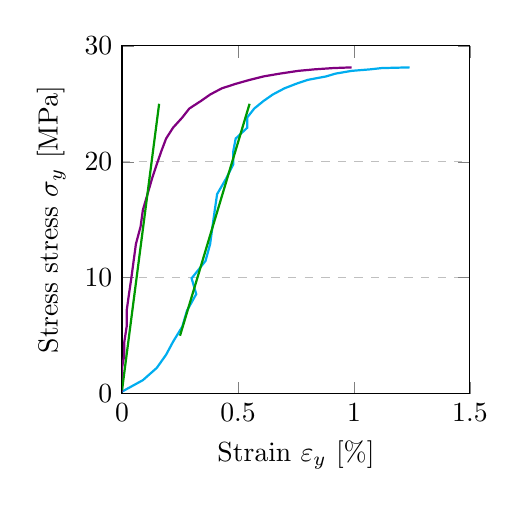
\begin{tikzpicture}
		\pgfplotstableread{
		stress	areaoi	totarea
		0.18	0.00	0.00
		1.17	0.09	0.00
		2.23	0.15	0.00
		3.36	0.19	0.01
		4.48	0.22	0.01
		5.79	0.26	0.02
		7.16	0.28	0.02
		8.59	0.32	0.03
		9.95	0.30	0.04
		11.45	0.36	0.05
		12.92	0.38	0.06
		14.41	0.39	0.08
		15.85	0.40	0.09
		17.21	0.41	0.11
		18.59	0.45	0.13
		19.79	0.48	0.15
		20.94	0.48	0.17
		22.00	0.49	0.19
		22.94	0.54	0.22
		23.82	0.54	0.26
		24.59	0.57	0.29
		25.24	0.61	0.34
		25.80	0.65	0.38
		26.33	0.70	0.43
		26.72	0.75	0.49
		27.06	0.80	0.55
		27.36	0.88	0.61
		27.60	0.92	0.68
		27.84	0.99	0.76
		27.97	1.07	0.83
		28.08	1.12	0.91
		28.14	1.24	0.99
		
		}\datatable
		
		
		
		
		\begin{axis}[no markers,
		name=plot0,height=6cm,width=6cm,
		    xlabel={Strain $\varepsilon_y$ [\%]},
		    ylabel={Stress stress $\sigma_y$ [MPa]},
		    xmin=0, xmax=1.5,
		    ymin=0, ymax=30,
		%     xtick={0,...,5},
		%    ytick={0,20,40,60,80},
		%     xticklabels={$0$,$0.2$,$0.4$,$0.6$,$0.8$, $1$}, 
		%     x tick label style={yshift=-1ex,
		%     rotate=45,anchor=east},
		    ymajorgrids=true,
		    grid style=dashed,
		]
		% \end{axis}    
		% \begin{axis}[legend pos=outer north east]
		 
		 
		    \addplot [thick, cyan] table[x=areaoi,y=stress] {\datatable}; \label{ex1}
		%     \addlegendentry{Total surface area}
		    \addplot [thick, violet	] table[x=totarea,y=stress] {\datatable};
		    \label{ex2}
		%     \addlegendentry{Surface area of interest}
			\addplot [thick, green!60!black] coordinates {(0.0, 0.3) (0.16,25.0)};
			\addplot [thick, green!60!black] coordinates {(0.25, 5) (0.55,25.0)};
			
		
		\end{axis}
		
		\end{tikzpicture}		
        \caption{}
        \label{fig:explot}
    \end{subfigure}

\caption{a) Barelling formation on initial cubic shape. b) DIC image of
\textit{Vasa} oak specimen during compressive testing including displacement
field $(mm)$. c) Experimental strain vs.
stress curves for \textit{Vasa} oak  specimen, chosen surface area of interest(\ref{ex1}) and
total area of surface (\ref{ex2})}
\label{fig:threegraphs}
\end{figure}












\begin{description}
\item{\textit{Model}}
\end{description}

\begin{figure}[h]
\centering
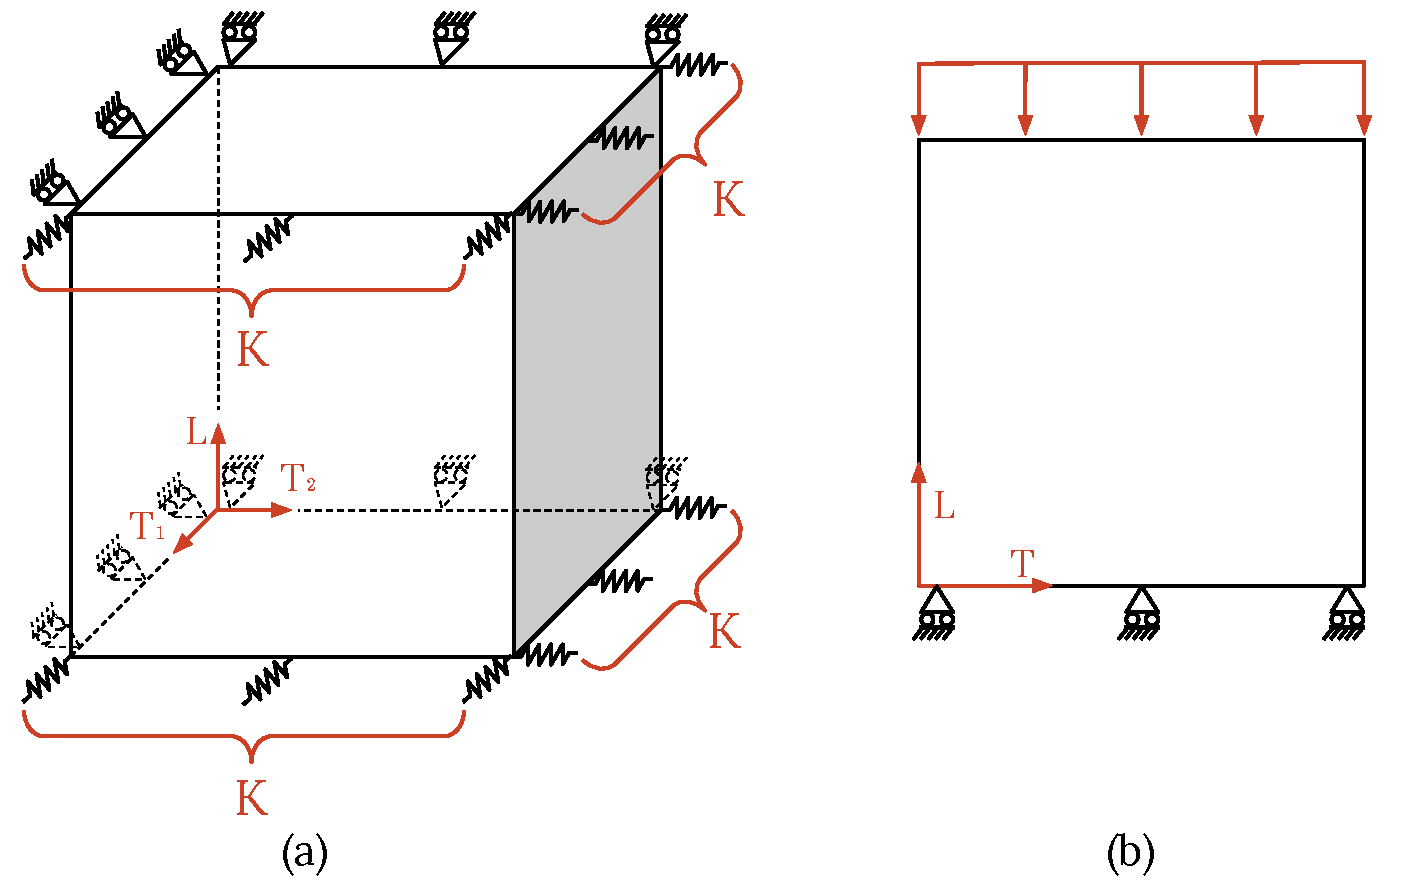
\includegraphics[width=8cm]{BarellingPaper.pdf}
\label{fig:Barrelling}
\caption{\label{fig:Barrelling} Finite element model of cubic specimen}
\end{figure}



The finite element program COMSOL Multiphysics 4.4 \cite{Comsol} was used for
the experimental simulations.
A cube (Figure \ref{fig:Barrelling})  with unity dimensions was modeled with
3D solid elements.
The platens of universal testing machine were not included in the model.
Instead, the compressive loading was simulated as a downward vertical prescribed
displacement. The magnitude of this prescribed displacement was set to 0.01
which corresponds to  1\%  of  strain respectively.

A \textit{Free Quad} mesh was placed on a top surface and swept throughout
the whole geometry using \textit{Quadrilateral} meshing method which generates
hexahedrons. We have solved the model using different number of FE. 
After a mesh refinement study, a $10\times10\times10$ mesh of quadratic
elements was determined to provide reasonably accurate results for the purpose of this study.

The friction between platens and specimen is the main reason for the
barrelling formation \cite{Narayanasamy198821, kulkarni1969}. To simulate that
friction we have introduced friction parameters $K$ that were applied to the
mutually orthogonal edges on the top and the bottom surface of the cube (Figure
\ref{fig:Barrelling}).

\begin{description}
\item{\textit{Material input parameters}}
\end{description}

We simulated transverse isotropic and isotropic material behaviour.
The model was linear elastic. The material propeties are introduced in
Table \ref{table:simulpar}. A parametric values $a$ and $b$ were introduced in
order to vary between the two mechanical models. The first one is parametrising
the Young's modulus and the Poisson's ratio. The second one has been determined
numerically to parametrise the shear moduli values from
materials in Table \ref{table:nonlin}.
The orthotropic material was simulated with the imput parameters obtained from
the experiments \cite{vorobyevcharacterisation}.


\begin{description}
\item{\textit{Strain measuring methods}}
\end{description}

Three strain measuring cases were taken intro accont in simulation.
In the \textit{first} case,  the average strain from the total area surface was
obtained and used as a value for obtaining axial stiffness $E_1$. In the
\textit{second} case, the 50\% of cube surface (Figure \ref{fig:experiment}) was used to calculate the
 average strain. The area was chosen in order to disregard the ``clamping''
 effect. Finally in the \textit{third} method the strain is measured between two
 points in the center of the specimen as it is suggested in ASTM code \cite{american2009standard}.


\begin{description}
\item[{\color {red}Conclusions for the model}]
\end{description}


\begin{center}% note that \centering uses less vspace...
\begin{figure}[!ht]
\pgfplotsset{every axis legend/.append style={
		at={(0.5,1.03)},
		anchor=north}}

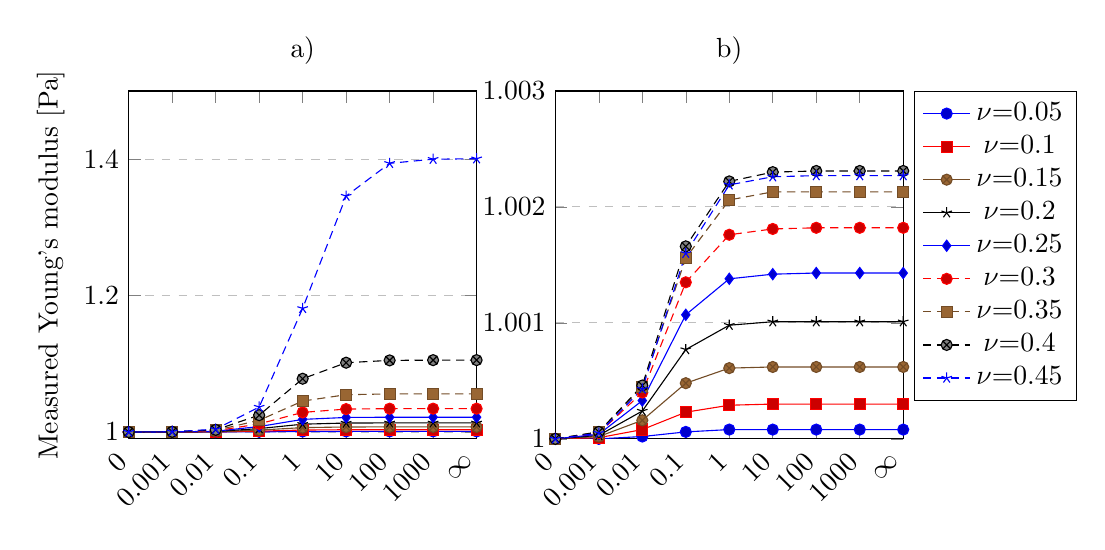
\begin{tikzpicture}[scale=1]

	\pgfplotstableread{
	K	0.05	0.1	0.15	0.2	0.25	0.3	0.35	0.4	0.45
1	1	1	1	1	1	1	1	1	1
2	1.00001	1.00002	1.00004	1.00008	1.00013	1.00018	1.00025	1.00033	1.00042
3	1.00005	1.00019	1.00043	1.00076	1.00121	1.00174	1.00241	1.00319	1.00412
4	1.00032	1.00127	1.00283	1.00505	1.00802	1.01194	1.01722	1.02472	1.03666
5	1.00075	1.00292	1.00645	1.0115	1.01853	1.02879	1.04539	1.07813	1.18128
6	1.00087	1.00335	1.0074	1.01319	1.02137	1.03365	1.0547	1.10164	1.34588
7	1.00089	1.00341	1.00751	1.01339	1.0217	1.03423	1.05589	1.10502	1.39391
8	1.00089	1.00341	1.00752	1.0134	1.02174	1.03429	1.05602	1.10538	1.39995
9	1.00089	1.00341	1.00752	1.01341	1.02174	1.0343	1.05603	1.10542	1.40064
}\datatable

\pgfplotstableread{
K	0.05	0.1	0.15	0.2	0.25	0.3	0.35	0.4	0.45
1	1	1	1	1	1	1	1	1	1
2	1	1.00001	1.00002	1.00003	1.00004	1.00005	1.00006	1.00006	1.00005
3	1.00002	1.00008	1.00016	1.00024	1.00033	1.0004	1.00045	1.00046	1.00043
4	1.00006	1.00023	1.00048	1.00077	1.00107	1.00135	1.00156	1.00166	1.0016
5	1.00008	1.00029	1.00061	1.00098	1.00138	1.00176	1.00206	1.00222	1.00219
6	1.00008	1.0003	1.00062	1.00101	1.00142	1.00181	1.00213	1.0023	1.00226
7	1.00008	1.0003	1.00062	1.00101	1.00143	1.00182	1.00213	1.00231	1.00227
8	1.00008	1.0003	1.00062	1.00101	1.00143	1.00182	1.00213	1.00231	1.00227
9	1.00008	1.0003	1.00062	1.00101	1.00143	1.00182	1.00213	1.00231	1.00227

}\datatableA




\begin{axis}[
name=plot0,height=6cm,width=6cm,
    title={a)},
%    xlabel={Temperature [\textcelsius]},
    ylabel={Measured Young's modulus [Pa]},
    xmin=1, xmax=9,
    ymin=0.99, ymax=1.5,
    xtick={1,...,9},
%    ytick={0,20,40,60,80},
    xticklabels={$0$,$0.001$,$0.01$,$0.1$,$1$, $10$, $100$,
    $1000$, $\infty$}, 
    x tick label style={yshift=-1ex,
    rotate=45,anchor=east},
    ymajorgrids=true,
    grid style=dashed,
]
% \end{axis}    
% \begin{axis}[legend pos=outer north east]
 
 
    \addplot table[x=K,y=0.05] {\datatable};
%     \addlegendentry{$\nu$=0.05}
    \addplot table[x=K,y=0.1] {\datatable};
%     \addlegendentry{$\nu$=0.1}
    \addplot table[x=K,y=0.15] {\datatable};
%     \addlegendentry{$\nu$=0.15}
    \addplot table[x=K,y=0.2] {\datatable};
%     \addlegendentry{$\nu$=0.2}
    \addplot table[x=K,y=0.25] {\datatable};
%     \addlegendentry{$\nu$=0.25}
    \addplot table[x=K,y=0.3] {\datatable};
%     \addlegendentry{$\nu$=0.3}
    \addplot table[x=K,y=0.35] {\datatable};
%     \addlegendentry{$\nu$=0.35}
    \addplot table[x=K,y=0.4] {\datatable};
%     \addlegendentry{$\nu$=0.4}
    \addplot table[x=K,y=0.45] {\datatable};
%     \addlegendentry{$\nu$=0.45}
\end{axis}

\begin{axis}[legend pos=outer north east,
	name=plot2,at={($(plot0.east)+(1cm,0)$)},anchor=west, height=6cm,width=6cm,
    title={b)},
%    xlabel={Temperature [\textcelsius]},
%    ylabel={Measured stiffness [Pa]},
    xmin=1, xmax=9,
    ymin=1, ymax=1.003,
    yticklabel style={/pgf/number format/fixed,
                  /pgf/number format/precision=3},
    xtick={1,...,9},
%    ytick={0,20,40,60,80},
    xticklabels={$0$,$0.001$,$0.01$,$0.1$,$1$, $10$, $100$,
    $1000$, $\infty$}, 
    x tick label style={yshift=-1ex,
        rotate=45,anchor=east},
    ymajorgrids=true,
    grid style=dashed,
    bar shift=0pt
]

	\addplot table[x=K,y=0.05] {\datatableA};
    \addlegendentry{$\nu$=0.05}
    \addplot table[x=K,y=0.1] {\datatableA};
    \addlegendentry{$\nu$=0.1}
    \addplot table[x=K,y=0.15] {\datatableA};
   \addlegendentry{$\nu$=0.15}
    \addplot table[x=K,y=0.2] {\datatableA};
    \addlegendentry{$\nu$=0.2}
    \addplot table[x=K,y=0.25] {\datatableA};
    \addlegendentry{$\nu$=0.25}
    \addplot table[x=K,y=0.3] {\datatableA};
    \addlegendentry{$\nu$=0.3}
    \addplot table[x=K,y=0.35] {\datatableA};
    \addlegendentry{$\nu$=0.35}
    \addplot table[x=K,y=0.4] {\datatableA};
    \addlegendentry{$\nu$=0.4}
    \addplot table[x=K,y=0.45] {\datatableA};
   \addlegendentry{$\nu$=0.45}


\end{axis}


\end{tikzpicture}


\captionsetup{justification=centering}
\caption{Relations between Young's modulus and spring
coefficient \textit{K} for a) isotropic material and b) transverse isotropic
[\textit{a=0.1}] material with different Poisson's ratios.}
\end{figure}

\end{center}

\begin{center}
\begin{figure}[!ht]
\pgfplotsset{every axis legend/.append style={
		at={(0.5,1.03)},
		anchor=north}}

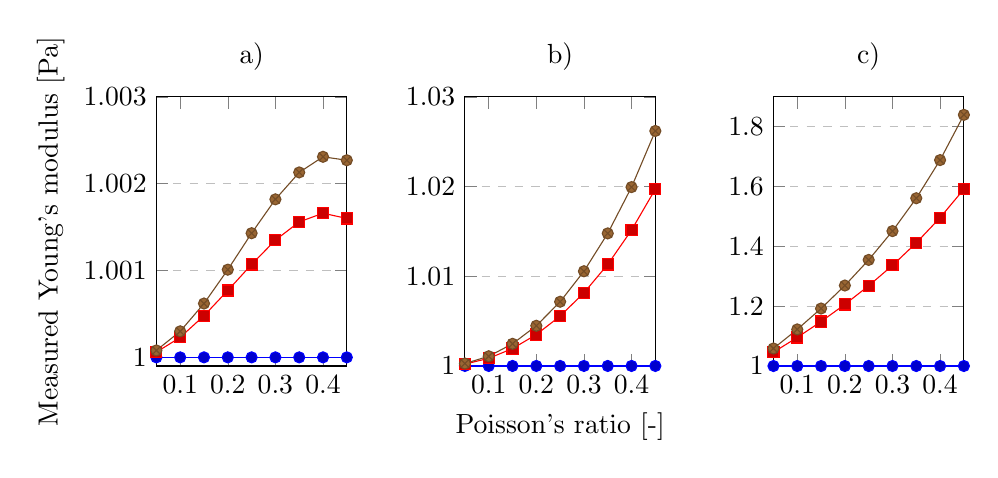
\begin{tikzpicture}[scale=1]

\pgfplotstableread{
nuxy	tr0	tr0.1	trINF
0.05	1	1.00006	1.00008
0.1	1	1.00023	1.0003
0.15	1	1.00048	1.00062
0.2	1	1.00077	1.00101
0.25	1	1.00107	1.00143
0.3	1	1.00135	1.00182
0.35	1	1.00156	1.00213
0.4	1	1.00166	1.00231
0.45	1	1.0016	1.00227

}\totarea

\pgfplotstableread{
nuxy	tr0	tr0.1	trINF	
0.05	1	1.00021	1.00027
0.1	1	1.00085	1.00108
0.15	1	1.00194	1.00247
0.2	1	1.0035	1.00448
0.25	1	1.00556	1.00716
0.3	1	1.00815	1.01056
0.35	1	1.01132	1.01478
0.4	1	1.01515	1.01994
0.45	1	1.01972	1.0262

}\chosenarea

\pgfplotstableread{
nuxy	tr0	tr0.1	trINF
0.05	1	1.04613	1.05867
0.1	1	1.09553	1.12248
0.15	1	1.14863	1.19228
0.2	1	1.20598	1.26922
0.25	1	1.26828	1.35482
0.3	1	1.33646	1.45114
0.35	1	1.41178	1.56104
0.4	1	1.49596	1.6886
0.45	1	1.59142	1.83986


}\experiment


%plot transv iso total area DSP

\begin{axis}[
name=b1,height=5cm,width=4cm,
    title={a)},
%    xlabel={Temperature [\textcelsius]},
    ylabel={Measured Young's modulus [Pa]},
    xmin=0.05, xmax=0.45,
    ymin=0.9999, ymax=1.003,
        yticklabel style={/pgf/number format/fixed,
                  /pgf/number format/precision=3},
%     xtick={1,...,9},
%    ytick={0,20,40,60,80},
%     xticklabels={$K=0$,$K=0.001$,$K=0.01$,$K=0.1$,$K=1$, $K=10$, $K=100$,
%     $K=1000$, $K=\infty$}, 
%     x tick label style={
%     rotate=60,anchor=east},
    ymajorgrids=true,
    grid style=dashed,
]
% \end{axis}    
% \begin{axis}[legend pos=outer north east]
 
 
    \addplot table[x=nuxy,y=tr0	] {\totarea}; \label{k1}
%     \addlegendentry{$\nu$=0.05}
    \addplot table[x=nuxy,y=tr0.1 ] {\totarea}; \label{k2}
%     \addlegendentry{$\nu$=0.1}
    \addplot table[x=nuxy,y=trINF ] {\totarea}; \label{k3}
%     \addlegendentry{$\nu$=0.15}

\end{axis}


%plot transviso chosen area  DSP

\begin{axis}[legend pos=outer north east,
	name=b2,at={($(b1.east)+(1.5cm,0)$)},anchor=west, height=5cm, width=4cm,
    title={b)},
    xlabel={Poisson's ratio [-]},
%    ylabel={Measured stiffness [Pa]},
    xmin=0.05, xmax=0.45,
    ymin=0.99999, ymax=1.03,
    yticklabel style={/pgf/number format/fixed,
                  /pgf/number format/precision=4},
%     xtick={1,...,9},
%    ytick={0,20,40,60,80},
%     xticklabels={$K=0$,$K=0.001$,$K=0.01$,$K=0.1$,$K=1$, $K=10$, $K=100$,
%     $K=1000$, $K=\infty$},
%     x tick label style={
%         rotate=60,anchor=east},
    ymajorgrids=true,
    grid style=dashed,
%     scaled y ticks=base 10:3,
    bar shift=0pt
]

    \addplot table[x=nuxy,y=tr0	] {\chosenarea}; \label{k1}
%     \addlegendentry{$\nu$=0.05}
    \addplot table[x=nuxy,y=tr0.1 ] {\chosenarea}; \label{k2}
%     \addlegendentry{$\nu$=0.1}
    \addplot table[x=nuxy,y=trINF ] {\chosenarea}; \label{k3}
%     \addlegendentry{$\nu$=0.15}

%Experimental approach

\end{axis}


\begin{axis}[legend pos=outer north east,
	name=b3,at={($(b2.east)+(1.5cm,0)$)},anchor=west, height=5cm,width=4cm,
    title={c)},
%    xlabel={Temperature [\textcelsius]},
%    ylabel={Measured stiffness [Pa]},
    xmin=0.05, xmax=0.45,
    ymin=0.9999, ymax=1.9,
    yticklabel style={/pgf/number format/fixed,
                  /pgf/number format/precision=3},
%     xtick={1,...,9},
%    ytick={0,20,40,60,80},
%     xticklabels={$K=0$,$K=0.001$,$K=0.01$,$K=0.1$,$K=1$, $K=10$, $K=100$,
%     $K=1000$, $K=\infty$},
%     x tick label style={
%         rotate=60,anchor=east},
    ymajorgrids=true,
    grid style=dashed,
    bar shift=0pt
]

    \addplot table[x=nuxy,y=tr0	] {\experiment}; \label{k1}
%     \addlegendentry{$\nu$=0.05}
    \addplot table[x=nuxy,y=tr0.1 ] {\experiment}; \label{k2}
%     \addlegendentry{$\nu$=0.1}
    \addplot table[x=nuxy,y=trINF ] {\experiment}; \label{k3}
%     \addlegendentry{$\nu$=0.15}




\end{axis}


\end{tikzpicture}
\captionsetup{justification=centering}
\caption{Measured stiffness vs. given Poisson's ratio
($\nu_{31}$, $\nu_{32}$) in transverse-isotropic material for spring
coefficients $K=0$ (\ref{k1}), $K=0.1$ (\ref{k2}) and $K=\infty$ (\ref{k3});\\
\color{red}{a) chosen area of interest , b) total area of interest c)
experiment.}}


\end{figure}
\end{center}







\section{Results and Discussions}
\begin{itemize}
\color{red}
\item What were the findings?

	\begin{enumerate}
	\color{black}
		\item Barellling formation is less in transverse isotropic and orthotropic
		material.
		\item The larger the Poisson�s ratio in isotropic materials, the more severe
		the barrelling.
		\item Barelling effect does not significant for the transverse isotropic
		material
		\item 3 measuring methods were compared {\color{red} add the plots}
	\end{enumerate}
\end{itemize}


%poisson's vs poisson's dependency
\color{black}

\begin{center}
\begin{figure}[!ht]
\pgfplotsset{every axis legend/.append style={
		at={(0.5,1.03)},
		anchor=north}}

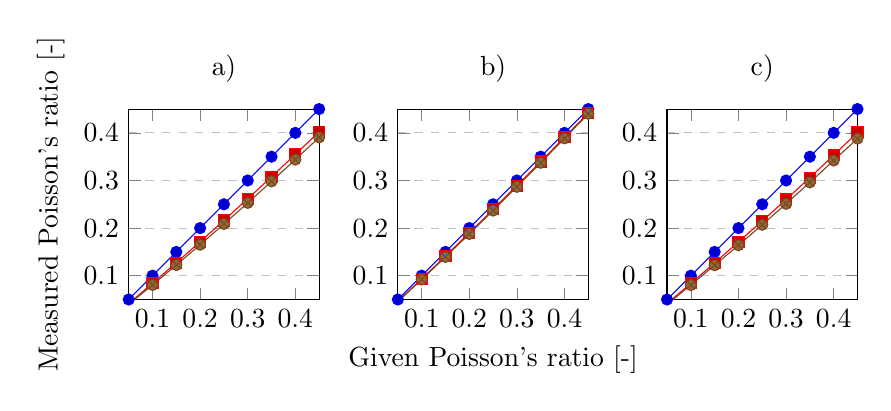
\begin{tikzpicture}[scale=1]

\pgfplotstableread{
nuxy	tr0	tr0.1	trINF	i0	i0.1	iINF
0.05	0.05	0.04161	0.03981	0.05	0.04691	0.04119
0.1	0.1	0.08404	0.08063	0.1	0.0942	0.08349
0.15	0.15	0.12728	0.1224	0.15	0.14194	0.1269
0.2	0.2	0.1713	0.16507	0.2	0.1902	0.17142
0.25	0.25	0.21607	0.2086	0.25	0.23904	0.21698
0.3	0.3	0.26158	0.25295	0.3	0.28856	0.26348
0.35	0.35	0.30782	0.29808	0.35	0.33888	0.31078
0.4	0.4	0.35479	0.34396	0.4	0.39023	0.35826
0.45	0.45	0.40251	0.39058	0.45	0.44309	0.39141

}\nutotarea

\pgfplotstableread{
nuxy	tr0	tr0.1	trINF	i0	i0.1	iINF
0.05	0.05	0.0463	0.0455	0.05	0.04906	0.04728
0.1	0.1	0.09342	0.09201	0.1	0.09847	0.09552
0.15	0.15	0.14133	0.13944	0.15	0.14821	0.1447
0.2	0.2	0.18995	0.18774	0.2	0.19829	0.19481
0.25	0.25	0.23926	0.23685	0.25	0.24866	0.24584
0.3	0.3	0.28918	0.28671	0.3	0.29933	0.29782
0.35	0.35	0.33969	0.33727	0.35	0.35026	0.35076
0.4	0.4	0.39072	0.38847	0.4	0.40142	0.40477
0.45	0.45	0.44224	0.44027	0.45	0.45283	0.46032
}\nuchosenarea

\pgfplotstableread{
nuxy	tr0	tr0.1	trINF	i0	i0.1	iINF
0.05	0.05	0.0416	0.03970	0.05	0.04690	0.04090
0.1	0.1	0.0839	0.08040	0.1	0.09410	0.08250
0.15	0.15	0.127	0.12200	0.15	0.14200	0.12500
0.2	0.2	0.171	0.16400	0.2	0.19000	0.16800
0.25	0.25	0.215	0.20700	0.25	0.23900	0.21300
0.3	0.3	0.26	0.25100	0.3	0.28800	0.26000
0.35	0.35	0.306	0.29600	0.35	0.33900	0.30900
0.4	0.4	0.353	0.34200	0.4	0.39000	0.36200
0.45	0.45	0.401	0.38800	0.45	0.44300	0.41900

}\nuexperiment




\begin{axis}[
name=c1,height=4cm,width=4cm,
    title={a)},
%    xlabel={Temperature [\textcelsius]},
    ylabel={Measured Poisson's ratio [-]},
    xmin=0.05, xmax=0.45,
    ymin=0.05, ymax=0.45,
        yticklabel style={/pgf/number format/fixed,
                  /pgf/number format/precision=3},
%     xtick={1,...,9},
%    ytick={0,20,40,60,80},
%     xticklabels={$K=0$,$K=0.001$,$K=0.01$,$K=0.1$,$K=1$, $K=10$, $K=100$,
%     $K=1000$, $K=\infty$}, 
%     x tick label style={
%     rotate=60,anchor=east},
    ymajorgrids=true,
    grid style=dashed,
]
% \end{axis}    
% \begin{axis}[legend pos=outer north east]
 
 
    \addplot table[x=nuxy,y=tr0	] {\nutotarea}; \label{nuk1}
%     \addlegendentry{$\nu$=0.05}
    \addplot table[x=nuxy,y=tr0.1 ] {\nutotarea}; \label{nuk2}
%     \addlegendentry{$\nu$=0.1}
    \addplot table[x=nuxy,y=trINF ] {\nutotarea}; \label{nuk3}
%     \addlegendentry{$\nu$=0.15}

\end{axis}


% plot transviso chosen area  DSP

\begin{axis}[legend pos=outer north east,
	name=c2,at={($(c1.east)+(1cm,0)$)},anchor=west, height=4cm, width=4cm,
    title={b)},
    xlabel={Given Poisson's ratio [-]},
%    ylabel={Measured stiffness [Pa]},
    xmin=0.05, xmax=0.45,
    ymin=0.05, ymax=0.45,
%     yticklabel style={/pgf/number format/fixed,
%                   /pgf/number format/precision=3},
%     xtick={1,...,9},
%    ytick={0,20,40,60,80},
%     xticklabels={$K=0$,$K=0.001$,$K=0.01$,$K=0.1$,$K=1$, $K=10$, $K=100$,
%     $K=1000$, $K=\infty$},
%     x tick label style={
%         rotate=60,anchor=east},
    ymajorgrids=true,
    grid style=dashed,
    bar shift=0pt
]

    \addplot table[x=nuxy,y=tr0	] {\nuchosenarea}; \label{nuk1}
%     \addlegendentry{$\nu$=0.05}
    \addplot table[x=nuxy,y=tr0.1 ] {\nuchosenarea}; \label{nuk2}
%     \addlegendentry{$\nu$=0.1}
    \addplot table[x=nuxy,y=trINF ] {\nuchosenarea}; \label{nuk3}
%     \addlegendentry{$\nu$=0.15}

%Experimental approach

\end{axis}


\begin{axis}[legend pos=outer north east,
	name=c3,at={($(c2.east)+(1cm,0)$)},anchor=west, height=4cm,width=4cm,
    title={c)},
%    xlabel={Temperature [\textcelsius]},
%    ylabel={Measured stiffness [Pa]},
    xmin=0.05, xmax=0.45,
    ymin=0.05, ymax=0.45,
%     yticklabel style={/pgf/number format/fixed,
%                   /pgf/number format/precision=3},
%     xtick={1,...,9},
%    ytick={0,20,40,60,80},
%     xticklabels={$K=0$,$K=0.001$,$K=0.01$,$K=0.1$,$K=1$, $K=10$, $K=100$,
%     $K=1000$, $K=\infty$},
%     x tick label style={
%         rotate=60,anchor=east},
    ymajorgrids=true,
    grid style=dashed,
    bar shift=0pt
]

    \addplot table[x=nuxy,y=tr0	] {\nuexperiment}; \label{nuk1}
%     \addlegendentry{$\nu$=0.05}
    \addplot table[x=nuxy,y=tr0.1 ] {\nuexperiment}; \label{nuk2}
%     \addlegendentry{$\nu$=0.1}
    \addplot table[x=nuxy,y=trINF ] {\nuexperiment}; \label{nuk3}
%     \addlegendentry{$\nu$=0.15}




\end{axis}


\end{tikzpicture}
\captionsetup{justification=centering}
\caption{Measured vs. given Poisson's ratio
($\nu_{31}$, $\nu_{32}$) in transverse-isotropic material for spring
coefficients $K=0$ (\ref{k1}), $K=0.1$ (\ref{k2}) and $K=\infty$ (\ref{k3});\\
\color{red}{a) total area of interest, b) chosen area of interest c)
experiment.}}


\end{figure}
\end{center}

\begin{figure}[!ht]
\centering
\pgfplotsset{every axis legend/.append style={
		at={(0.5,1.03)},
		anchor=north}}

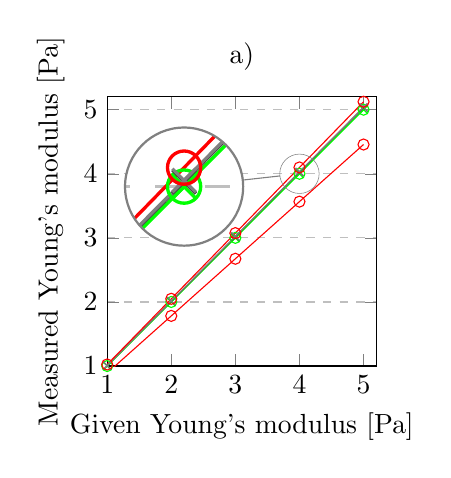
\begin{tikzpicture}
 [spy using outlines={circle,black,magnification=3,size=1cm,
 connect spies}]
% Data for the plot showing the stability and independency of Emod

\pgfplotstableread{
Emodgiven	nul	tr0.1	iso0.1	trinf	isoinf
1	1	1.00638	1.02469	1.00797	0.89131
2	2	2.01276	2.04938	2.01595	1.78262
3	3	3.01914	3.07408	3.02392	2.67393
4	4	4.02551	4.09877	4.0319	3.56524
5	5	5.03189	5.12346	5.03987	4.45655
}\emodgivread



\begin{axis}[
name=c1,height=5cm,width=5cm,
    title={a)},
    xlabel={Given Young's modulus [Pa]},
    ylabel={Measured Young's modulus [Pa]},
    xmin=1, xmax=5.2,
    ymin=1, ymax=5.2,
        yticklabel style={/pgf/number format/fixed,
                  /pgf/number format/precision=3},
%     xtick={1,...,9},
%    ytick={0,20,40,60,80},
%     xticklabels={$K=0$,$K=0.001$,$K=0.01$,$K=0.1$,$K=1$, $K=10$, $K=100$,
%     $K=1000$, $K=\infty$}, 
%     x tick label style={
%     rotate=60,anchor=east},
    ymajorgrids=true,
    grid style=dashed,
]

    \addplot[mark=otimes, green, solid] table[x=Emodgiven,y=nul	]
    {\emodgivread};
    \label{e1}
%     \addlegendentry{$\nu$=0.05}
    \addplot [mark=x, darkgray,    ] table[x=Emodgiven,y=tr0.1 ]
    {\emodgivread}; \label{e2}
%     \addlegendentry{$\nu$=0.1}
    \addplot [mark=x, gray,  ] table[x=Emodgiven,y=trinf ]
    {\emodgivread};
    \label{e3}
%     \addlegendentry{$\nu$=0.15}
    \addplot [mark=o, red  ] table[x=Emodgiven,y=iso0.1 ]
    {\emodgivread};
    \label{e4}
%     \addlegendentry{$\nu$=0.1}
    \addplot [mark=o, red    ] table[x=Emodgiven,y=isoinf ]
    {\emodgivread};
    \label{e5}
%     \addlegendentry{$\nu$=0.15}

\coordinate (spypoint) at (axis cs:4,4);
\coordinate (magnifyglass) at (axis cs:2.2,3.8);

\end{axis}

% \spy on (2.5,2.5) in node [left] at (1.25,1.75);
\spy [gray, size=1.5cm] on (spypoint)
   in node[fill=white] at (magnifyglass);

\end{tikzpicture}
\captionsetup{justification=centering}
\caption{Measured vs. given stiffness
($E_{1}$) in transverse-isotropic(\ref{e2}) and isotropic(\ref{e4}) material for
spring coefficients $K=0$ (\ref{e1}), $K=0.1$ (\ref{e2}, \ref{e4}) and
$K=\infty$ (\ref{e3}, \ref{e5});\\
\color{red}{a) total area of interest, b) chosen area of interest c)
experiment.}}


\end{figure}




\color{red}
\begin{itemize}
\item Use diagrams and/or tables, objective and truthful presentation
\item Results and discussion distinguishable
\item New and old results and discussion
\end{itemize}


\section{Conclusions}

\section*{Acknowledgements}

\section*{References}

\pagebreak


\section*{Tables}
\it{\color{red}Add the description for the parameters in the tables}

\begin{description}

\item[]
\begin{sidewaystable}[!htbp]\
\caption{Engineering constants used in model} % title of Table
\centering % used for centering table
\begin{tabular}{c c c c c c c c c c c c} % centered columns (4 columns)
\hline\hline %inserts double horizontal lines
 $E_{1}$ (GPa) & $E_{2}$ (GPa) & $E_{3}$ (GPa) & $G_{31}$ (GPa) &
$G_{21}$ (GPa) & $G_{32}$ (GPa) & $\nu_{31}$ & $\nu_{21}$ & $\nu_{32}$ &
$\nu_{13}$ & $\nu_{12}$ & $\nu_{23}$ \\ % inserts table heading

\hline % inserts single horizontal line
$E$ & $E$ & $a\cdot{E}$ & $\frac{(b\cdot(a-1)+1)\cdot{E}}{2(1+\nu)}$  &
$\frac{a\cdot{E}}{2(1+\nu)}$ & $\frac{(b\cdot(a-1)+1)\cdot{E}}{2(1+\nu)}$ & $\nu$ & $\nu$ & $\nu$ & $\frac{\nu}{a}$ & $\nu$ & $\frac{\nu}{a}$ \\
% inserting body of the table
[1ex] % [1ex] adds vertical space
\hline %inserts single lines

\multicolumn{6}{l}{%
  \begin{minipage}{9cm}%
\tiny Note: $E=1$; $\nu=0.25$; Parameter $a=1$ for isotropic and $a=10$
    for transverse-isotropic material model; Shear stiffness parameter 
    $b=1$ for isotropic and for transverse-isotropic
    $b=[0.1,2,3]$.
      \end{minipage}%
}\\
      
	
\end{tabular}

\label{table:simulpar} % is used to refer this table in the text
\end{sidewaystable}

\item[]
\begin{sidewaystable}[!htbp]\
\caption{Typical engineering properties of transverse-isotropic materials\cite{hyer2009stress}} % title of Table
\centering % used for centering table
\begin{tabular}{l c c c } % centered columns (4 columns)
\hline\hline %inserts double horizontal lines

& Graphite-polymer composite \cite{hyer2009stress}  & Glass-polymer composite
\cite{hyer2009stress} & Archaeoligical wood \cite{vorobyevcharacterisation}\\
%  & $E_{1}$  & $E_{2}$ (GPa) & $E_{3}$ (GPa) & $\nu_{12}$ & $\nu_{13}$
% & $\nu_{23}$ & $G_{12}$ (GPa) & $G_{13}$ (GPa) & $G_{23}$ (GPa) \\ % inserts
% % table heading

\hline % inserts single horizontal line

$E_{1}$ (GPa) & 12.10 & 15.20 & 0.60\\
$E_{2}$ (GPa) & 12.10 & 15.20 & 0.35\\
$E_{3}$ (GPa) & 155.0 & 50.00 & 6.75\\

$G_{31}$ (GPa) & 4.40 & 4.70 & 0.62\\
$G_{21}$ (GPa) & 3.20 & 3.28 & 0.14\\
$G_{32}$ (GPa) & 4.40 & 4.70 & 0.33\\

$\nu_{31}$ (-) & 0.248 & 0.254 & 0.37\\
$\nu_{21}$ (-) & 0.458 & 0.428 & 0.30\\
$\nu_{32}$ (-) & 0.248 & 0.254 & 0.69\\





% Graphite-polymer composite & 12.10 &  & 12.10 & 155.0 & 0.458 & 0.248 & 0.248 &
% 0.6 & 0.72 & 0.72\\
% % inserting body of the table
% Transverse isotropic & 1.49 & $E_1=E_2$ & 12.14 & 0.66 & 0.06 & 0.04 & 0.2 &
%  0.6 & 0.72\\
% Isotropic & - & - & 12.14 \\
\hline %inserts single line
\end{tabular}
\label{table:nonlin} % is used to refer this table in the text
\end{sidewaystable}
\end{description}


\it{\color{red}Check whether i need to add the isotropic parameters and transv
ortho}


%%%%%%%%%%% VIDEO CAPTIONS

%% If submitting video's as a supplement to the manuscript, include only the video captions here (not the figures).  Videos are uploaded separately in the online Elsevier Editorial Submission process.  If videos are not included, comment out this section.

%% Do not remove the page break here.
\pagebreak

\bibliography{mybibfile}

\end{document}
